%% ------------------------------------------------------------------------- %%
\chapter{Distribuci�n Beta}
\label{cap:conceptos}

Introducci�n al cap�tulo

%% ------------------------------------------------------------------------- %%
\section{Distribuci�n Beta}
\label{sec:dbeta}

Una clase de distribuciones que permite modelar variables continuas limitadas al intervalo $(0,1)$ es la distribuci�n beta.

%% ------------------------------------------------------------------------- %%
\subsection{Funci�n de densidad de probabilidad}
\label{sec:fdpbeta}
la funci�n de densidad de probabilidad de una variable aleat�ria $Y$ que sigue una distribuci�n beta es dada por

\begin{equation}
f_{Y}(y\mid \alpha,\beta)=\frac{\Gamma(\alpha+\beta)}{\Gamma(\alpha)\Gamma(\beta)}
y^{\alpha-1}(1-y)^{\beta-1}, \ \ \ 0 < y < 1. \label{densidad}
\end{equation}


\noindent Esta distribuci�n es bastante flexible para modelar este tipo de datos debido a que su funci�n de densidad de probabilidad puede tomar diversas formas dependiendo del valor de los par�metros que caracterizan a esta distribuci�n (ver figura \ref{densidades}). 

\begin{figure}[!htb]
\begin{center}
%\framebox{
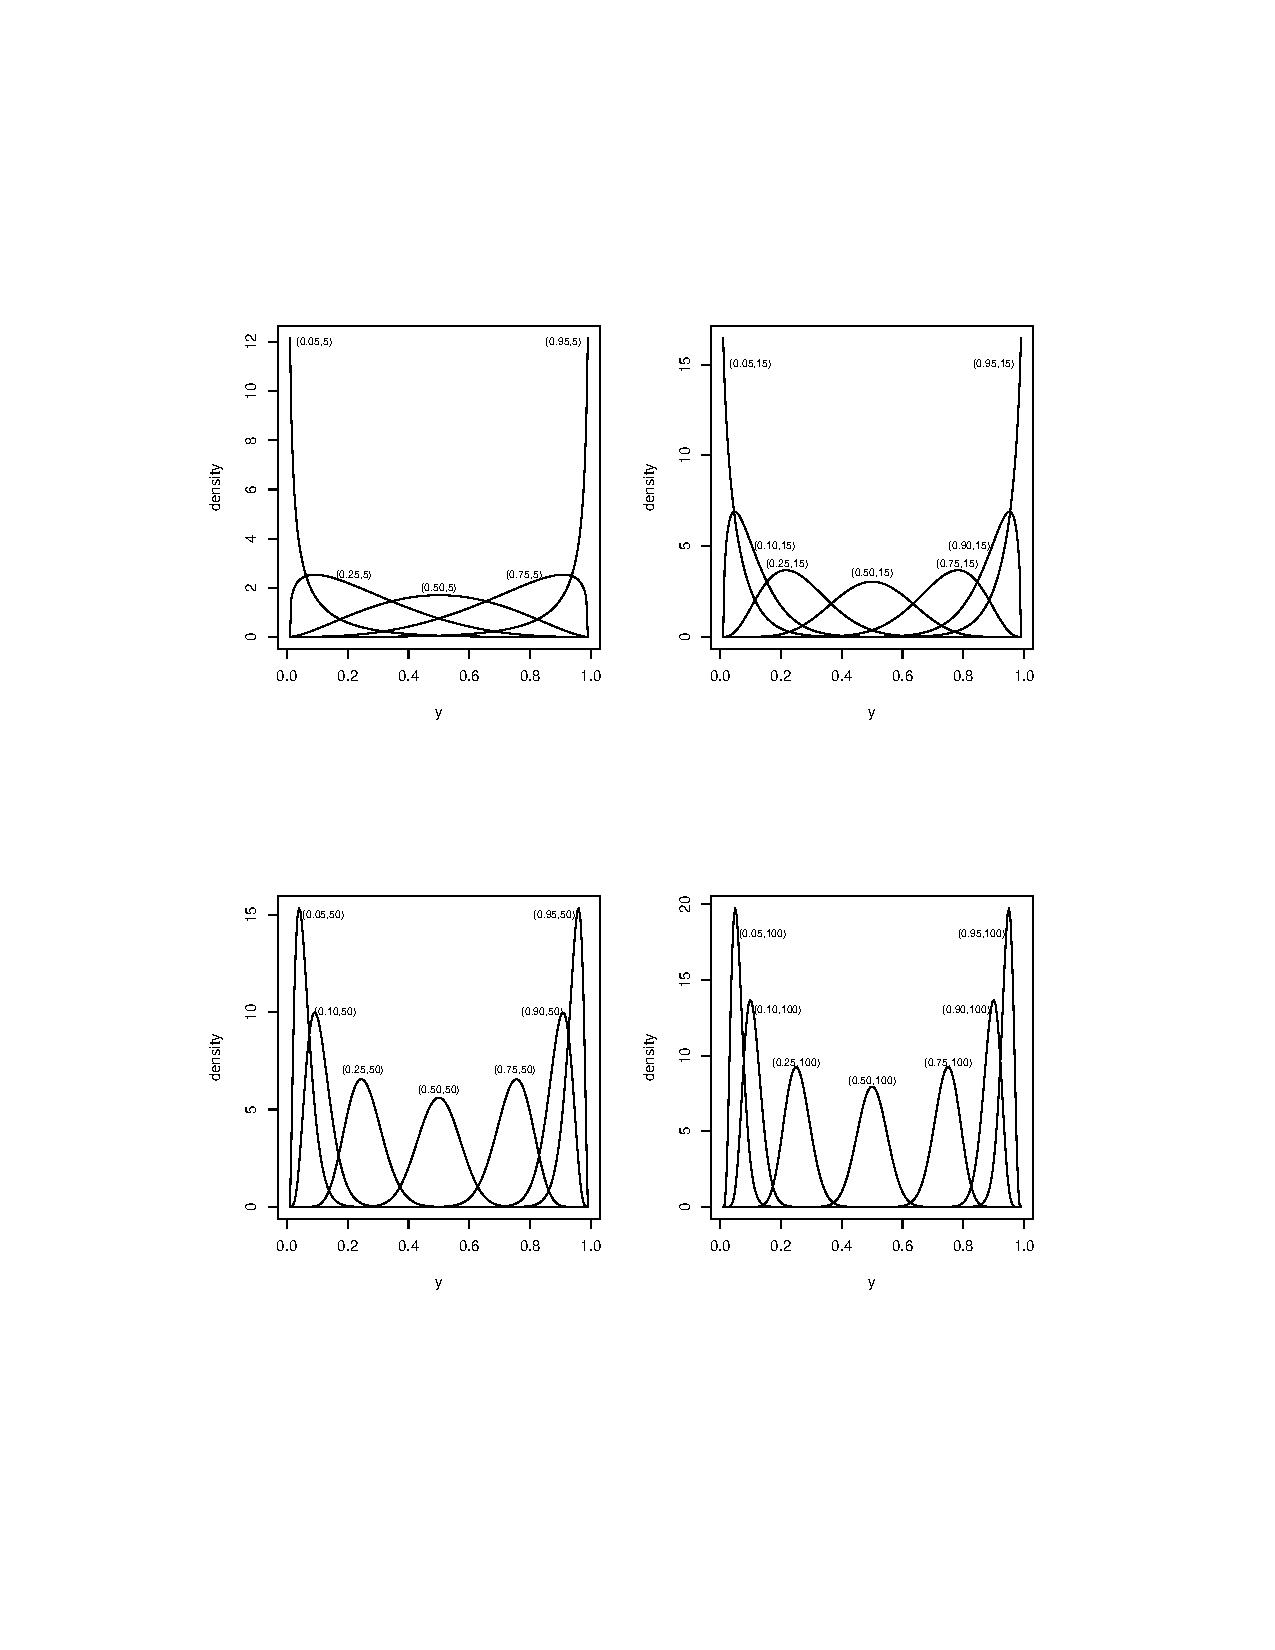
\includegraphics[scale=.80]{densidades}
%}
\caption{Densidades de la distribuci�n beta para diferentes valores de los par�metros}
\label{densidades}
\end{center}
\end{figure}

%% ------------------------------------------------------------------------- %%
\subsection{Propiedades}
\label{sec:betaprop}


\noindent La media y la variancia de una distribuci�n son expresadas por
\begin{equation}
E(y)=\frac{\alpha} {\alpha + \beta} \ \ \ \ \mbox{y}\ \ \ \  Var(y)=\frac{\alpha \beta}{(\alpha+\beta)^2(\alpha+\beta+1)}.\label{mv}
\end{equation}



\section{Parametrizaci�n alternativa}
\label{sec:paralter}

Por este motivo, recientemente en la literatura han sido propuestos modelos de regresi�n basados en esta distribuci�n, por ejemplo ver \citet{betareg}. El modelo propuesto por estos autores permite la interpretaci�n de los par�metros en t�rminos de la respuesta en su escala original (variable respuesta sin transformar). Ellos consideran una reparametrizaci�n del modelo donde $\mu = \alpha / (\alpha + \beta)$ y $\phi=\alpha + \beta$, y de (\ref{mv}) obtenemos que 

\begin{equation}
E(y)=\mu \ \ \ \ \mbox{y}\ \ \ \  Var(y)=\frac{V(\mu)}{1+\phi}
\end{equation}

\noindent donde $V(\mu)=\mu(1-\mu)$, as� tenemos que $\mu$ es la media de la variable respuesta y $\phi$ puede ser interpretado como un par�metro de precisi�n. Luego, en la nueva parametrizaci�n la densidad de la distribuci�n beta puede ser escrita como

\begin{equation}
f_{Y}(y\mid \mu,\phi)=\frac{\Gamma(\phi)}{\Gamma(\mu\phi)\Gamma((1-\mu)\phi)}
y^{\mu\phi-1}(1-y)^{(1-\mu)\phi-1}, \ \ \ 0 < y < 1. \label{densidad2}
\end{equation}

\noindent donde $0<\mu<1$ y $\phi>0$.


